\documentclass{report}
\usepackage{graphicx, tikz-cd, float, titlepic, booktabs} % Required for inserting images
\usepackage{pgfplots}
\usepackage{multicol}
\usepackage{makecell}
\pgfplotsset{compat=1.15}
\usepackage{mathrsfs}
\usetikzlibrary{arrows}
\usepackage{amsmath, amssymb, amsthm, amsfonts, siunitx, physics, gensymb}
\AtBeginDocument{\RenewCommandCopy\qty\SI}
\usepackage[version=4]{mhchem}
\usepackage[most,many,breakable]{tcolorbox}
\usepackage{xcolor, fancyhdr, varwidth}
\usepackage[Glenn]{fncychap}
%Options: Sonny, Lenny, Glenn, Conny, Rejne, Bjarne, Bjornstrup
\usepackage{hyperref, cleveref}
\usepackage{icomma, enumitem} %comma as decimal and continue enumerate with [resume]
\usepackage{plimsoll} %use standard state symbol with \stst
\usepackage[danish]{babel}
\renewcommand{\cellalign}{cl}
\renewcommand{\theadalign}{cl}
\renewcommand\theadfont{\bfseries}
%%%%%%%%%%%%%%%%%%%%%%%%%%%%%%
% SELF MADE COLORS
%%%%%%%%%%%%%%%%%%%%%%%%%%%%%%
\definecolor{myg}{RGB}{56, 140, 70}
\definecolor{myb}{RGB}{45, 111, 177}
\definecolor{myr}{RGB}{199, 68, 64}
\definecolor{mytheorembg}{HTML}{F2F2F9}
\definecolor{mytheoremfr}{HTML}{00007B}
\definecolor{mylenmabg}{HTML}{FFFAF8}
\definecolor{mylenmafr}{HTML}{983b0f}
\definecolor{mypropbg}{HTML}{f2fbfc}
\definecolor{mypropfr}{HTML}{191971}
\definecolor{myexamplebg}{HTML}{F2FBF8}
\definecolor{myexamplefr}{HTML}{88D6D1}
\definecolor{myexampleti}{HTML}{2A7F7F}
\definecolor{mydefinitbg}{HTML}{E5E5FF}
\definecolor{mydefinitfr}{HTML}{3F3FA3}
\definecolor{notesgreen}{RGB}{0,162,0}
\definecolor{myp}{RGB}{197, 92, 212}
\definecolor{mygr}{HTML}{2C3338}
\definecolor{myred}{RGB}{127,0,0}
\definecolor{myyellow}{RGB}{169,121,69}
\definecolor{myexercisebg}{HTML}{F2FBF8}
\definecolor{myexercisefg}{HTML}{88D6D1}
%%%%%%%%%%%%%%%%%%%%%%%%%%%%%%%%%%%%%%%%%%%%%%%%%%%%%%%%%%%%%%%%%%%%%%
% Box environments for theorems and problems
%%%%%%%%%%%%%%%%%%%%%%%%%%%%%%%%%%%%%%%%%%%%%%%%%%%%%%%%%%%%%%%%%%%%%
\setlength{\parindent}{1cm}
%================================
% Question BOX
%================================
\makeatletter
\newtcbtheorem{question}{Opgave}{enhanced,
	breakable,
	colback=white,
	colframe=myb!80!black,
	attach boxed title to top left={yshift*=-\tcboxedtitleheight},
	fonttitle=\bfseries,
	title={#2},
	boxed title size=title,
	boxed title style={%
			sharp corners,
			rounded corners=northwest,
			colback=tcbcolframe,
			boxrule=0pt,
		},
	underlay boxed title={%
			\path[fill=tcbcolframe] (title.south west)--(title.south east)
			to[out=0, in=180] ([xshift=5mm]title.east)--
			(title.center-|frame.east)
			[rounded corners=\kvtcb@arc] |-
			(frame.north) -| cycle;
		},
	#1
}{def}
\makeatother
%================================
% DEFINITION BOX
%================================

\newtheorem{defin}{Definition}[section] % Creates a new counter, number within section

\newtcbtheorem[number within=section, use counter*=defin]{Definition}{Definition}{enhanced,
	before skip=2mm,after skip=2mm, colback=red!5,colframe=red!80!black,boxrule=0.5mm,
	attach boxed title to top left={xshift=1cm,yshift*=1mm-\tcboxedtitleheight}, varwidth boxed title*=-3cm,
	boxed title style={frame code={
					\path[fill=tcbcolback]
					([yshift=-1mm,xshift=-1mm]frame.north west)
					arc[start angle=0,end angle=180,radius=1mm]
					([yshift=-1mm,xshift=1mm]frame.north east)
					arc[start angle=180,end angle=0,radius=1mm];
					\path[left color=tcbcolback!60!black,right color=tcbcolback!60!black,
						middle color=tcbcolback!80!black]
					([xshift=-2mm]frame.north west) -- ([xshift=2mm]frame.north east)
					[rounded corners=1mm]-- ([xshift=1mm,yshift=-1mm]frame.north east)
					-- (frame.south east) -- (frame.south west)
					-- ([xshift=-1mm,yshift=-1mm]frame.north west)
					[sharp corners]-- cycle;
				},interior engine=empty,
		},
	fonttitle=\bfseries,
	title={#2},#1}{def}

\newtcbtheorem[number within=section]{definition}{Definition}
{%
	enhanced,
	breakable,
	colback = red!5,
	frame hidden,
	boxrule = 0sp,
	borderline west = {2pt}{0pt}{solid, red!75!black},
	sharp corners,
	detach title,
	before upper = \tcbtitle\par\smallskip,
	coltitle = red!75!black,
	fonttitle = \bfseries\sffamily,
	description font = \mdseries,
	separator sign none,
	segmentation style={solid, red!75!black},
}
{th}

\newtcbtheorem{theo}%
    {Theorem}{}{theorem}
\newtcolorbox{prob}[1]{colback=red!5!white,colframe=red!50!black,fonttitle=\bfseries,title={#1}}

%================================
% NOTE BOX
%================================

\usetikzlibrary{arrows,calc,shadows.blur}
\tcbuselibrary{skins}
\newtcolorbox{note}[1][]{%
	enhanced jigsaw,
	colback=gray!20!white,%
	colframe=gray!80!black,
	size=small,
	boxrule=1pt,
	title=\textbf{Note:},
	halign title=flush center,
	coltitle=black,
	breakable,
	drop shadow=black!50!white,
	attach boxed title to top left={xshift=1cm,yshift=-\tcboxedtitleheight/2,yshifttext=-\tcboxedtitleheight/2},
	minipage boxed title=1.5cm,
	boxed title style={%
			colback=white,
			size=fbox,
			boxrule=1pt,
			boxsep=2pt,
			underlay={%
					\coordinate (dotA) at ($(interior.west) + (-0.5pt,0)$);
					\coordinate (dotB) at ($(interior.east) + (0.5pt,0)$);
					\begin{scope}
						\clip (interior.north west) rectangle ([xshift=3ex]interior.east);
						\filldraw [white, blur shadow={shadow opacity=60, shadow yshift=-.75ex}, rounded corners=2pt] (interior.north west) rectangle (interior.south east);
					\end{scope}
					\begin{scope}[gray!80!black]
						\fill (dotA) circle (2pt);
						\fill (dotB) circle (2pt);
					\end{scope}
				},
		},
	#1,
}
%================================
% EXAMPLE BOX
%================================
\newtcbtheorem[number within=section, use counter from=definition]{Example}{Example}
{%
	colback = myexamplebg
	,breakable
	,colframe = myexamplefr
	,coltitle = myexampleti
	,boxrule = 1pt
	,sharp corners
	,detach title
	,before upper=\tcbtitle\par\smallskip
	,fonttitle = \bfseries
	,description font = \mdseries
	,separator sign none
	,description delimiters parenthesis
}
{ex}
%================================
% THEOREM BOX
%================================

\tcbuselibrary{theorems,skins,hooks}
\newtcbtheorem[number within=section, use counter from=definition]{Theorem}{Theorem}
{%
	enhanced,
	breakable,
	colback = mytheorembg,
	frame hidden,
	boxrule = 0sp,
	borderline west = {2pt}{0pt}{mytheoremfr},
	sharp corners,
	detach title,
	before upper = \tcbtitle\par\smallskip,
	coltitle = mytheoremfr,
	fonttitle = \bfseries\sffamily,
	description font = \mdseries,
	separator sign none,
	segmentation style={solid, mytheoremfr},
}
{th}

%%%%%%%%%%%%%%%%%%%%%%%%%%%%%%%%%%%%%%%%%%%%%%%%%%%%%%%%%%%%%%%%%
% SELF MADE COMMANDS
%%%%%%%%%%%%%%%%%%%%%%%%%%%%%%
\newcommand{\sol}{\setlength{\parindent}{0cm}\textbf{\textit{Løsning:}}\setlength{\parindent}{1cm}}
%%%%%%%%%%%%%%%%%%%%%%%%%%%%%%%%%
\usepackage[tmargin=2cm,rmargin=1in,lmargin=1in,margin=0.85in,bmargin=2cm,footskip=.2in]{geometry}\pagestyle{fancy}
\lhead{Minrui Kevin Zhou 3.b}
\rhead{Opgavesæt 8}

\title{Opgavesæt 8\\
{\Large \textbf{3.b kemi A}}}
\author{Kevin Zhou}
\date{\today}

\begin{document}
\maketitle
\begin{note}
  Databog fysik kemi (2007) er benyttet ved beregningerne.
\end{note}
\section*{Opgave 1: Et middel til behandling af bipolare lidelser}
\sol \\
\textbf{a.}
Massen af valproinsyre i opløsningen må være
\begin{equation*}
\begin{split}
  m(\text{valproinsyre} )&=M(\text{valproinsyre} ) \cdot n(\text{valproinsyre} )\\
  &=M(\text{valproinsyre}) \cdot c(\text{valproinsyre}) \cdot V\\
  &=144,21 \;\unit{g/mol} \cdot 0,0090 \;\unit{\textsc{m}} \cdot 0,100 \;\unit{L} \\
  &\approx 0,13 \;\unit{g} 
\end{split}
\end{equation*}
Massen af valproinsyre i opløsningen er altså $0,13 \;\unit{g} $. \\[1ex]
\textbf{b.}
Siden valproinsyre er svag, så har vi
\begin{equation*}
\begin{split}
  pH&=\frac{pK_s-\log\left(\frac{c_s}{\;\unit{\textsc{m}} }\right) }{2}\\
  &=\frac{4,8- \log\left(\frac{0,0090 \;\unit{\textsc{m}} }{\;\unit{\textsc{m}} }\right) }{2}\\
  &\approx 3,4
\end{split}
\end{equation*}
I den vandige opløsning af valproinsyre har vi altså $pH=3,4$.

\section*{Opgave 3: Cochenille - et farvestof udvundet af lus}
\sol \\
\textbf{a.} 
Hydroxygrupper bundet til et C-atom i en aromatisk ring tilhører stofklassen phenoler, og hydroxygrupper bundet til et alifatisk eller alicyclisk C-atom tilhører stofklassen alkoholer.
Dette er angivet for hver hydroxygruppe i strukturen for carminsyre i \cref{fig:carmin} (de blå tilhører stofklassen phenoler, og de røde tilhører stofklassen alkoholer).

\begin{figure}[H]
\begin{center}
  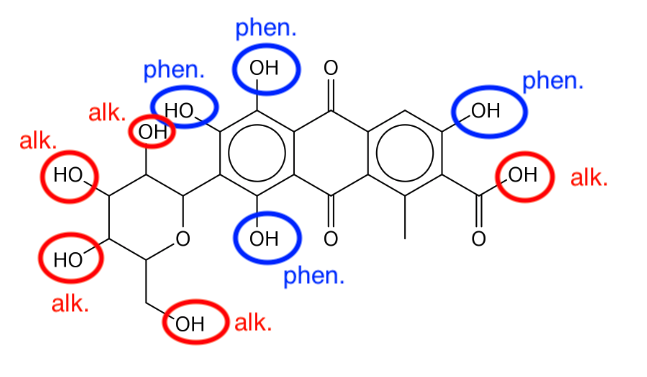
\includegraphics[width=0.8\textwidth]{carmin.png}
\end{center}
\caption{Hydroxygrupperne markeret i strukturen for carminsyre}
\label{fig:carmin}
\end{figure}

\noindent \textbf{b.}
Vi finder et udtryk for den molare absorptionskoefficient ud fra Lambert-Beers lov.
\begin{equation*}
\begin{split}
  A=\varepsilon _{\lambda } \cdot l \cdot [\text{carmin}] \iff \varepsilon _{\lambda } = \frac{A}{l \cdot [\text{carmin} ]}
\end{split}
\end{equation*}
Fra Excelfilen har vi, at når bølgelængden er $\lambda =515 \;\unit{nm} $, så er absorbansen $A=0,811$.
Vi indsætter da de kendte værdier og udregner den molare absorptionskoefficient.
\begin{equation*}
\begin{split}
  \varepsilon _{\lambda } &= \frac{A}{l \cdot [\text{carmin} ]}\\
  &=\frac{0,811}{1,00 \;\unit{cm} \cdot 1,00 \cdot 10 ^{-4} \;\unit{\textsc{m}} }\\
  &\approx 8,11 \cdot 10^3 \;\unit{\textsc{m}^{-1}\cdot cm ^{-1}} 
\end{split}
\end{equation*}
Den molare absorptionskoefficient for carmin ved bølgelængden 515 nm er altså $\varepsilon _{\lambda }=8,11 \cdot 10^3  \;\unit{\textsc{m}^{-1}\cdot cm ^{-1}} $.\\[1ex]
\textbf{c.}
Fra Lambert-Beers lov har vi, at 
\begin{equation*}
\begin{split}
  A=\varepsilon _{\lambda } \cdot l \cdot [\text{carmin}] &\iff [\text{carmin} ] = \frac{A}{l \cdot \varepsilon _{\lambda }}% \\
  %&\iff [\text{carmin} ] = k_0 \cdot A,
\end{split}
\end{equation*}
%hvor $k_0=\frac{1}{l \cdot \varepsilon _{\lambda }}$ er konstant. 
Hvis reaktionen er af 2. orden mht. carmin, så må der gælde, at 
\begin{equation*}
\begin{split}
  \frac{1}{[\text{carmin} ]} = k \cdot t + \frac{1}{[\text{carmin} ]_0} %&\iff \frac{\varepsilon _{\lambda } \cdot l}{A} = k \cdot t + \frac{\varepsilon _{\lambda } \cdot l}{A_0}
 %\frac{1}{k_0 \cdot A} = k \cdot t + \frac{1}{k_0 \cdot A_0}
\end{split}
\end{equation*}
%Siden $\varepsilon _{\lambda }$ og $l$ er konstante, så må $(t, \frac{\varepsilon _{\lambda } \cdot l}{A})$-grafen for reaktionen være en ret linje. 
Altså må $(t, \frac{1}{[\text{carmin} ]})$-grafen være en ret linje med hældningskoefficenten $k$, hvis reaktionen er af 2. orden mht. carmin.
Imidlertid har vi, at
\begin{equation*}
\begin{split}
\frac{1}{[\text{carmin} ]}&=\frac{\varepsilon _{\lambda } \cdot l}{A}\\
  &=\frac{1,00 \;\unit{cm} \cdot 8110 \;\unit{\textsc{m}^{-1}\cdot cm ^{-1}} }{A}\\
  &=\frac{8110 \;\unit{\textsc{m}^{-1}} }{A}
\end{split}
\end{equation*}
Vi laver da lineær regression på punkterne i $(t, \frac{1}{[\text{carmin} ]})$-grafen, hvilket ses i \cref{fig:t1carmin}.
\begin{figure}[H]
\begin{center}
  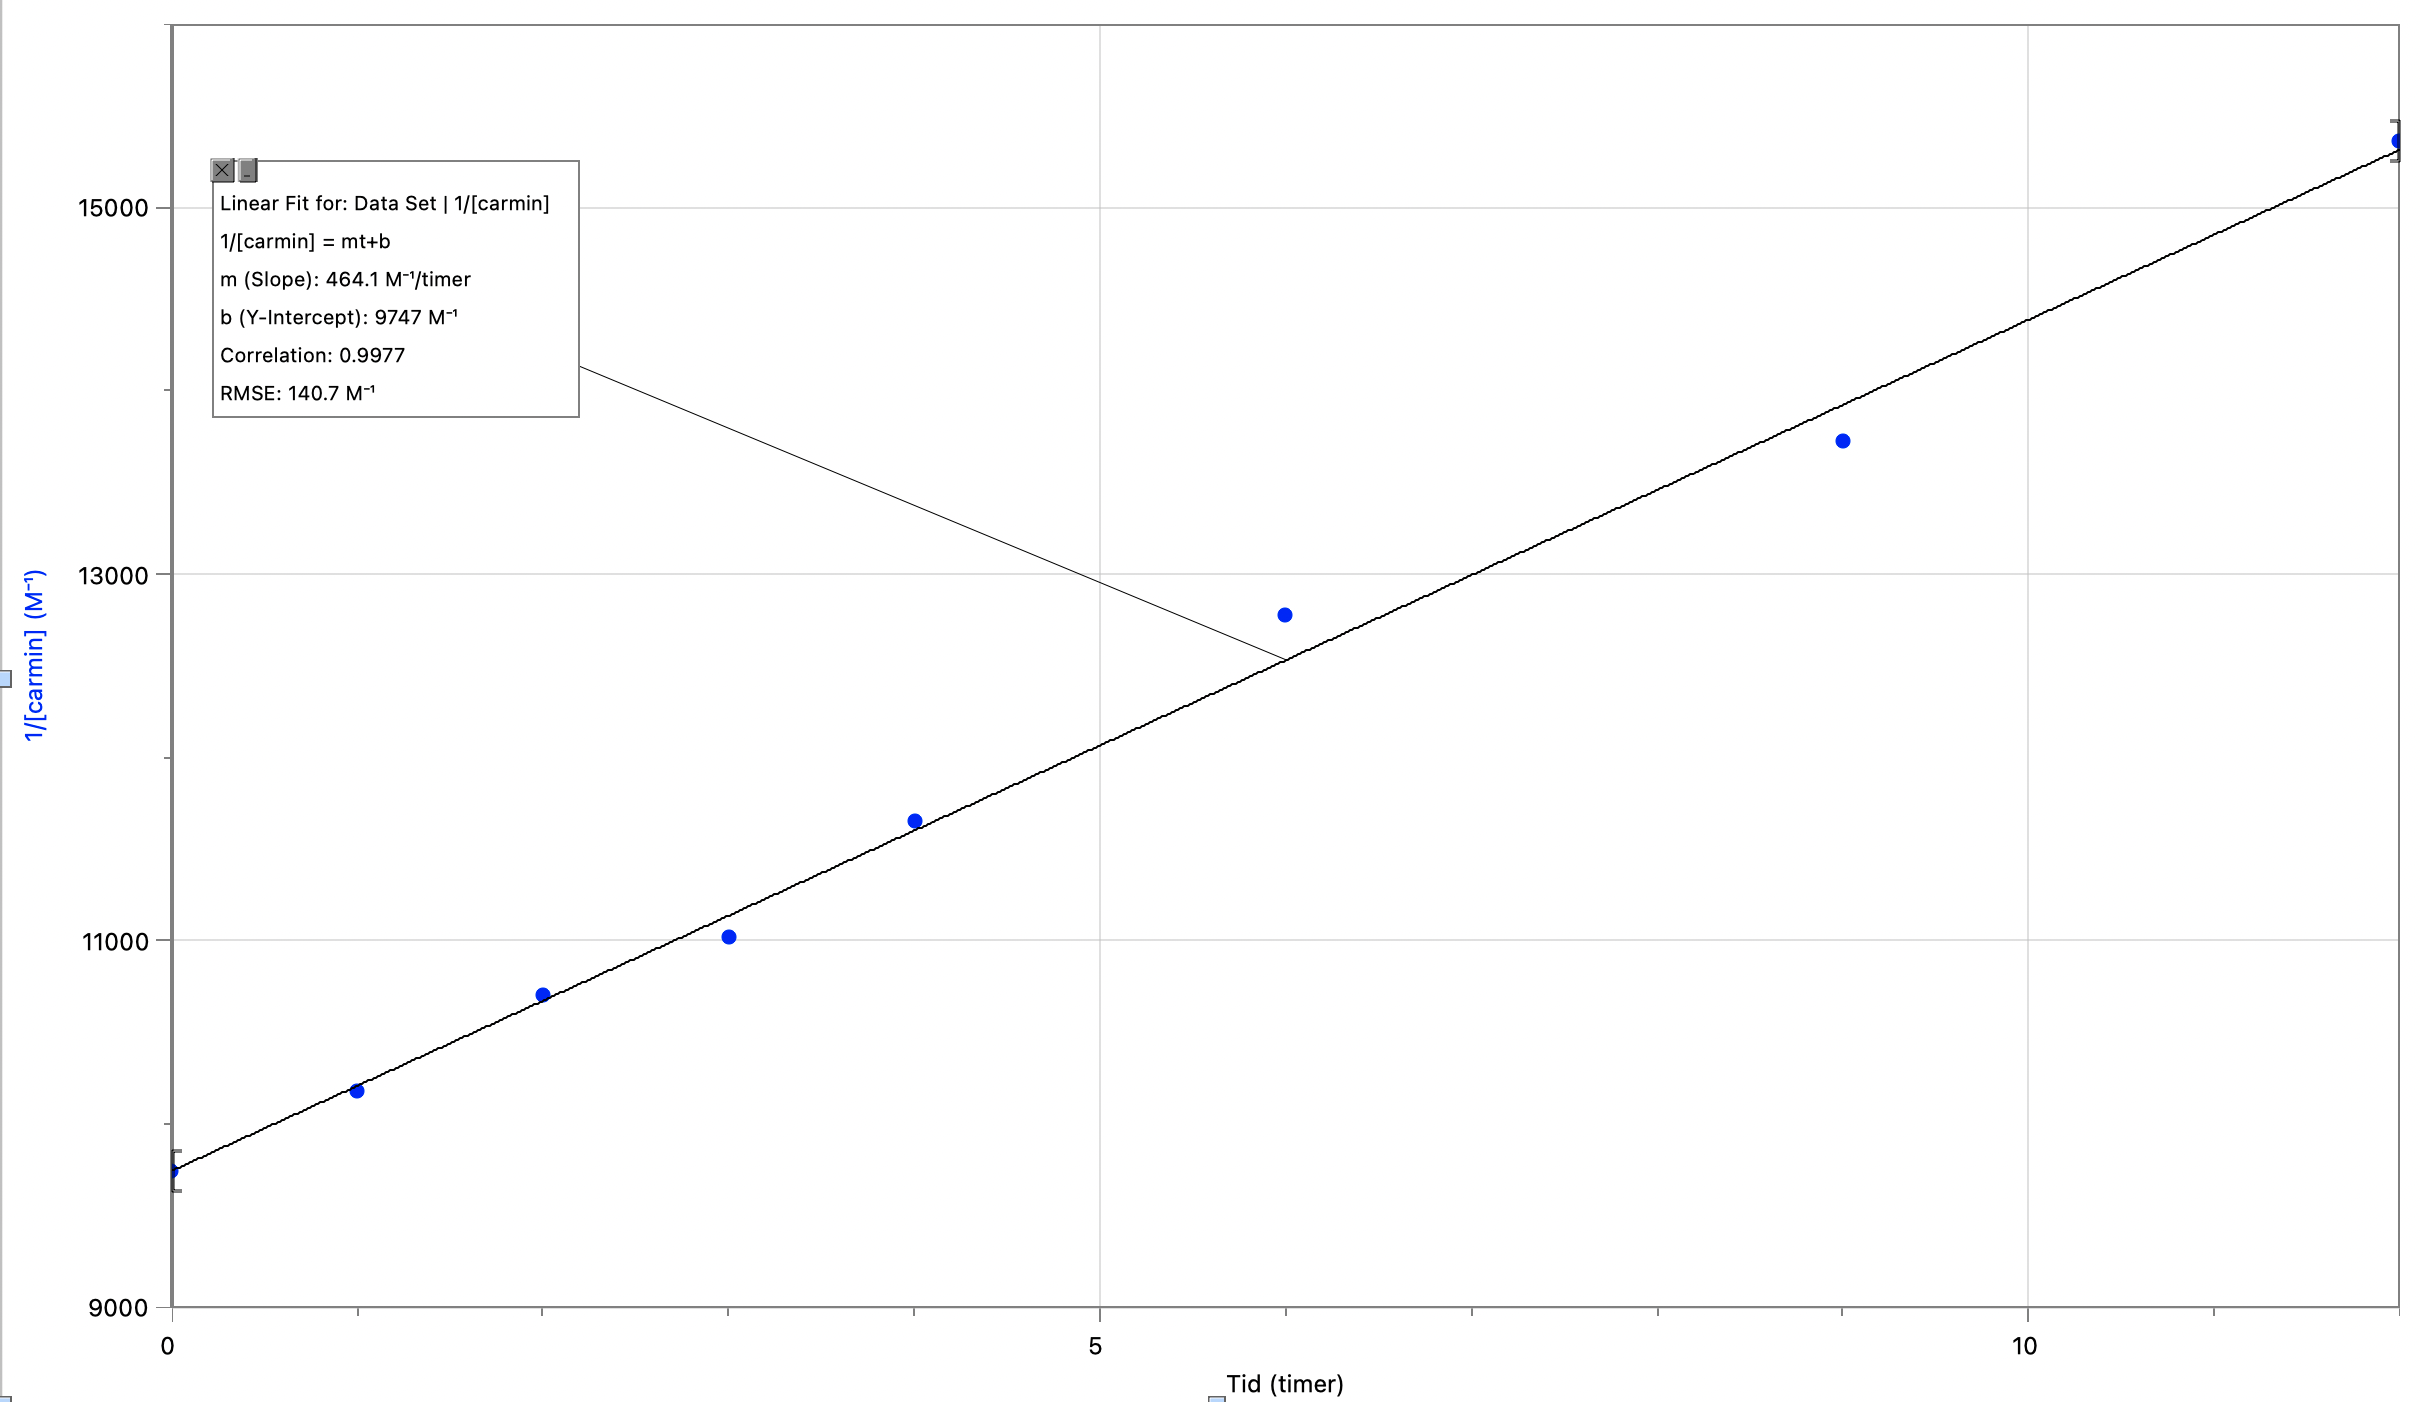
\includegraphics[width=0.8\textwidth]{t1carmin.png}
\end{center}
\caption{Lineær regression på $(t, \frac{1}{[\text{carmin} ]})$-grafen for reaktionen}
\label{fig:t1carmin}
\end{figure}
Vi ser, at punkterne tilnærmelsesvist følger den lineære sammenhæng.
Det vil sige, at nedbrydningen af carmin kan beskrives som en 2. ordens reaktion med hensyn til carmin.

Fra den lineære regression har vi, at funktionsudtrykket for nedbrydningen må være
\begin{equation*}
\begin{split}
  \frac{1}{[\text{carmin} ]}=464 \;\unit{\textsc{m}^{-1}\cdot h ^{-1}} + 9,75 \cdot 10^3 \;\unit{\textsc{m}^{-1}} 
\end{split}
\end{equation*}
hvor $h$ er enheden timer.\\[1ex]
\textbf{d.}
Der gælder, at fasen med octan-1-ol er upolær, hvor fasen med vand er polær.

Det er klart, at carminsyre i den neutrale form er den mindst polære.
For jo flere hydroner carminsyre afgiver, desto mere negativ og dermed mere polær bliver den så.
Med andre ord, har vi, at når pH vokser, så bliver carminsyre mere polær.
Altså bliver opløseligheden i vand større, når pH vokser.
Tilsvarende bliver opløseligheden i octan-1-ol mindre, når pH vokser.

Således må $D$ og derfor $\log\left(D\right) $ aftage, når pH vokser. 
Dette understøttes af figuren (se \cref{fig:D}), hvor $\log\left(D\right)$ er aftagende i hele intervallet. 
For at sætte nogle værdier på, har vi, at $\log\left(D\right) =1,1$ ved pH $=0$, og $\log\left(D\right) =-7,8$ ved pH $=12$. 
De fire "knæk" i grafen skyldes carminsyres evne til at afgive fire hydroner.
Bemærk, at disse knæk forekommer, hvor pH er omkring de givne p$K_s$-værdier.

\begin{figure}[H]
\begin{center}
  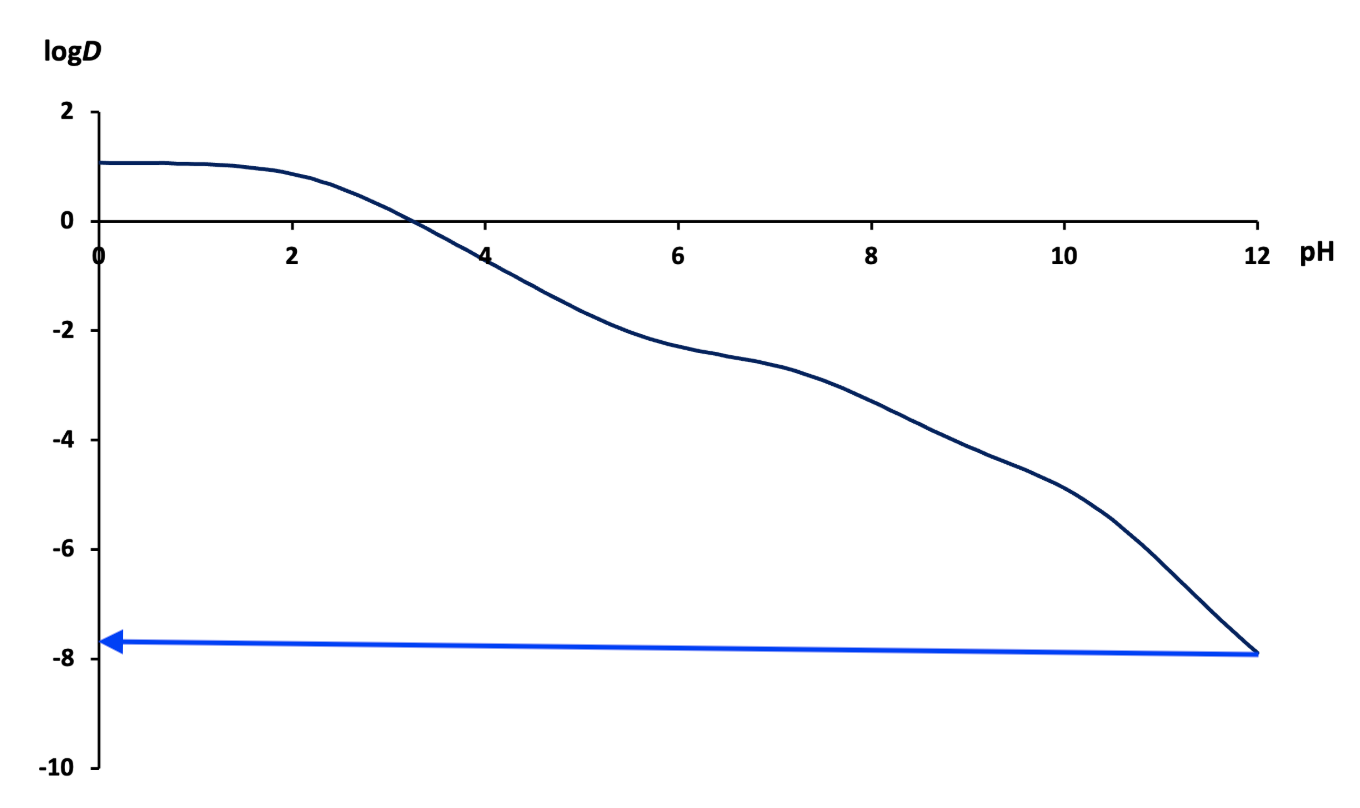
\includegraphics[width=0.8\textwidth]{logD.png}
\end{center}
  \caption{$(pH, \log\left(D\right) )$-graf for carminsyre}
\label{fig:D}
\end{figure}

\section*{Opgave 4: Iridium(IV)oxid - i højteknologiske materialer}
\sol \\
\textbf{a.}
Vi beregner stofmængden af dioxygen i beholderen med idealgasloven.
\begin{equation*}
\begin{split}
  n(\ce{O2} )&=\frac{p(\ce{O2} ) \cdot V}{R \cdot T}\\
  &=\frac{1,00 \;\unit{bar} \cdot 2,00 \;\unit{L} }{0,0831 \;\unit{\frac{L \cdot bar}{mol \cdot K}} \cdot 1325 \;\unit{K} }\\
  &\approx 0,0182 \;\unit{mol} 
\end{split}
\end{equation*}
Stofmængden af dioxygen i beholderen er altså $n(\ce{O2} )=0,0182 \;\unit{mol} $. \\[1ex]
\textbf{b.}
Vi starter med at opskrive ligevægtsloven for at bestemme ligevægtskonstantens enhed.
\begin{equation*}
\begin{split}
  K=\frac{1}{p(\ce{O2} )}
\end{split}
\end{equation*}
Det fremgår af ligevægtsloven, at enheden for $K$ må være $\unit{bar ^{-1}}$. 

\noindent Fra figuren i opgavebeskrivelsen har vi, at 
\begin{equation*}
\begin{split}
  \ln\left(K \cdot \unit{bar} \right) = 32968 \;\unit{K} \cdot \frac{1}{T} -22,813 \iff K=e^{32968 \;\unit{K} \cdot \frac{1}{T} -22,813}\;\unit{bar ^{-1}} 
\end{split}
\end{equation*}
Ligevægtskonstanten ved $1200 \;\unit{K} $ må da være 
\begin{equation*}
\begin{split}
  K&=e^{32968 \;\unit{K} \cdot \frac{1}{1200 \;\unit{K}} -22,813} \;\unit{bar ^{-1}} \\
  &\approx 105,7 \;\unit{bar ^{-1}} 
\end{split}
\end{equation*}
Ligevægtskonstanten ved 1200 K er altså $K=105,7 \;\unit{bar ^{-1}} $.\\[1ex]
\textbf{c.}
Fra van't Hoffs ligning har vi 
\[
\ln\left(K\right) =-\frac{\Delta H \stst }{R} \cdot \frac{1}{T} + \frac{\Delta S \stst }{R},
\] 
og fra figuren har vi 
\[
\ln\left(K \right) = 32968 \;\unit{K} \cdot \frac{1}{T} -22,813.
\] 
Ved kombination af ligningerne får vi 
\begin{equation*}
\begin{split}
  -\frac{\Delta H \stst }{R} = 32968 \;\unit{K} \iff \Delta H \stst = -R \cdot 32968 \;\unit{K}.
\end{split}
\end{equation*}
Vi får ligeledes
\begin{equation*}
\begin{split}
  \frac{\Delta S \stst }{R}= -22,813 \iff \Delta S \stst =-R \cdot 22,813
\end{split}
\end{equation*}
Vi udregner disse størrelser.
\begin{equation*}
\begin{split}
  \Delta H \stst &= -8,314 \;\unit{\frac{J}{mol \cdot K}}  \cdot 32968 \;\unit{K} \approx -2,7410 \cdot 10 ^{5} \;\unit{J/mol} \\
  \Delta S \stst &=-8,314 \;\unit{\frac{J}{mol \cdot K}}  \cdot 22,813 \approx -189,67 \;\unit{\frac{J}{mol \cdot K}} 
\end{split}
\end{equation*}
Der gælder, at en reaktion er spontan præcis når
\[
\Delta G < 0. 
\] 
Vi vil nu kontrollere, om det er tilfældet for reaktionen til tidspunktet $t _{\text{målt} }$:
\begin{equation*}
\begin{split}
  \Delta G &=\Delta G \stst + R \cdot T \cdot \ln\left(Y\right) \\
  &=-R \cdot T \cdot \ln\left(K\right)  + R \cdot T \cdot \ln\left(\frac{1}{p(\ce{O2} )}\right)\\
  &=R \cdot T \cdot \left(\ln\left(\frac{1}{p(\ce{O2} )}\right) - \ln\left(K\right) \right) \\
  &=R \cdot T \cdot \ln\left(\frac{1}{p(\ce{O2} ) \cdot K}\right)\\
  &=8,314 \;\unit{\frac{J}{mol \cdot K}} \cdot 1200 \;\unit{K} \cdot \ln\left(\frac{1}{0,15 \;\unit{bar} \cdot 105,7 \;\unit{bar ^{-1}} }\right) \\
  &\approx -2,757 \cdot 10 ^{4} \;\unit{J/mol} <0
\end{split}
\end{equation*}
Siden $\Delta G<0$ til tidspunktet $t _{\text{målt} }$, så må reaktionen altså være spontan. \\[1ex]
\textbf{d.}
Når ligevægten har indstillet sig, så må reaktionsbrøken være lig ligevægtskonstanten.
\begin{equation*}
\begin{split}
  K=\frac{1}{p(\ce{O2} )} \iff p(\ce{O2} )=\frac{1}{K}
\end{split}
\end{equation*}
Vi udregner nu $p(\ce{O2} )$.
\begin{equation*}
\begin{split}
  p(\ce{O2} )&=\frac{1}{7,91 \;\unit{bar ^{-1}} }\\
  &\approx 0,126 \;\unit{bar} 
\end{split}
\end{equation*}
Siden der ikke var noget iridium(IV)oxid i beholderen til start, så har vi 
\begin{equation*}
\begin{split}
  n(\ce{IrO2} )=-\Delta n(\ce{O2} ) &\iff m(\ce{IrO2} ) = -M(\ce{IrO2} ) \cdot \left(\frac{p_{\text{slut} }(\ce{O2}) \cdot V}{R \cdot T _{\text{slut} }} - \frac{p_{\text{start} }(\ce{O2}) \cdot V}{R \cdot T _{\text{ start}}}\right) \\
  &\implies  m(\ce{IrO2} ) = -M(\ce{IrO2} ) \cdot \frac{(p_{\text{slut} }(\ce{O2})-p_{\text{start}}(\ce{O2} )) \cdot V}{R \cdot T} 
\end{split}
\end{equation*}
Bemærk, at vi her har $T=T _{\text{start} }=T _{\text{slut} }$.
Vi udregner nu $m(\ce{IrO2} )$.
\begin{equation*}
\begin{split}
  m(\ce{IrO2} ) &= -M(\ce{IrO2} ) \cdot \frac{(p_{\text{slut} }(\ce{O2})-p_{\text{start}}(\ce{O2} )) \cdot V}{R \cdot T} \\
  &=-\left(192,2 \;\unit{g/mol} + 2 \cdot 16,00 \;\unit{g/mol} \right) \cdot \frac{(0,12642 \;\unit{bar} -1,00 \;\unit{bar} ) \cdot 2,00 \;\unit{L} }{0,0831 \;\unit{\frac{L \cdot bar}{mol \cdot K}} \cdot 1325 \;\unit{K}}\\
  &\approx 3,56 \;\unit{g} 
\end{split}
\end{equation*}
Massen af iridium(IV)oxid i beholderen ved ligevægt er altså $m(\ce{IrO2} )=3,56 \;\unit{g} $.
\end{document}
